% We adopt the presentation from~\cite{barr1990category}, where a category is viewed as an unlabeled directed graph~\autorefbrackets{def:cat} equipped with two additional functions and their associated properties. In this framework, a homomorphism~\autorefbrackets{def:cat:homo} is simply another term for an arrow. To enhance readability, we utilize the concepts of spans and cospans. After introducing the notion of a commutative diagram~\autorefbrackets{def:cat:diagram}, we proceed to define the pushout~\autorefbrackets{def:cat:po_pb}. The construction of pushouts in the category \textbf{Graph} is also explain.
% To establish the categorical foundations necessary for our work, we recall key concepts such as monomorphisms, spans, cospans, commutative diagrams, and pushouts, following the presentation in~\cite{barr1990category}. We then focus on pushouts with monomorphisms within the category of graphs.
% We follow the presentation in~\cite{barr1990category}. We then focus on pushouts with monomorphisms within the category of graphs.
 
% cat def
\begin{definition}[Category~\cite{pierce1991basic, barr1990category}]
    \label{def:cat}
    A \textbf{category} is an unlabeled graph \( C \) together with a total function \( u : C_0 \mathop{\to} C_1 \) and a partial function \( \star: C_1 \mathop{\times} C_1 \mathop{\to} C_1 \) such that 
        (i) for all edges \( f:X \mathop{\to} Y \) and \( g:Y \mathop{\to} Z \), the edge \( f \mathop{\star} g :X \mathop{\to} Z \) is defined; 
        (ii) for every node \( X \), \( u(X) \) is an edge from \( X \) to \( X \);
        (iii) for every \( f:X \mathop{\to} Y \), we have \(u(X) \mathop{\star} f \mathop{=} f \mathop{=} f \mathop{\star} u(Y)\);
        (iv) for all edges \( f \), \( g \) and \(h\), we have \( (f \mathop{\star} g) \mathop{\star} h \mathop{=} f \mathop{\star} (g \mathop{\star} h) \) whenever either side is defined.
    Edges are called \textbf{morphisms}. The function $\star$ is called \textbf{composition}. For all \( X \mathop{\in} C_0 \), the edge \( u(X) \) is denoted \( \operatorname{id}_X \) and is called the \textbf{identity} of the object \( X \).
    % \( C \) is called the \textbf{underlying graph} of the category \( \mathcal{C} \).
\end{definition} 

% cat notation * 
\begin{notation}
    The composition of morphisms \( f : X \to Y \) and \( g : Y \to Z \) is written in diagrammatic order as \( f \star g \), rather than in functional order \( g \circ f \). 
    % The advantage is that, when reading from left to right, the morphisms appear in the same order as in the corresponding diagram, making the notation more intuitive for visual reasoning.
\end{notation}  

\begin{definition}[Monomorphism \cite{pierce1991basic,barr1990category}]
    \label{def:cat:homo}
    A morphism \( f : X \to Y \) is \textbf{monic} (or a \textbf{monomorphism}) if for all morphisms \( g \) and \( h \), if \( g \star f = h \star f \), then \( g = h \). A monomorphism is denoted by \( f : X \rightarrowtail Y \).
\end{definition} 

\begin{example}
    \trackedtext{Finite edge-labeled directed multigraphs} and their homomorphisms form a category, hereafter denoted \textbf{Graph}. Its objects are labeled graphs, its morphisms are graph homomorphisms, and the monomorphisms are injective homomorphisms.
\end{example}

%span
\begin{definition}[Span \cite{lowe2010graph}]
    A pair \( (\alpha : A \mathop{\to} B,~\beta : A \mathop{\to} C) \) of morphisms with a common domain is called a \textbf{span}, denoted by \( B \overset{\alpha}{\leftarrow} A \overset{\beta}{\rightarrow} C \).
\end{definition}
%cospan
\begin{definition}[Cospan]
    An ordered pair \( (\beta' : B \to D,~\alpha' : C \to D) \) of morphisms with a common codomain is called a \textbf{cospan}, denoted by \( B \overset{\beta'}{\rightarrow} D \overset{\alpha'}{\leftarrow} C \). 
\end{definition} 
%diagram 

\begin{definition}[Diagram~\cite{barr1990category}]
    \label{def:cat:diagram}
    Let \( G \) be an unlabeled graph. A \textbf{diagram} (in \( \mathcal{C} \) of shape \( G \)) is a homomorphism of unlabeled graphs \( h : G \to C \) where \( C \) is the underlying unlabeled graph of the category \( \mathcal{C} \). A diagram is \textbf{commutative} if, for all nodes \( u \), \( v \), and any two paths from \( u \) to \( v \) in the unlabeled graph \( G \):

    \begin{center}
    \resizebox{12cm}{!}{
        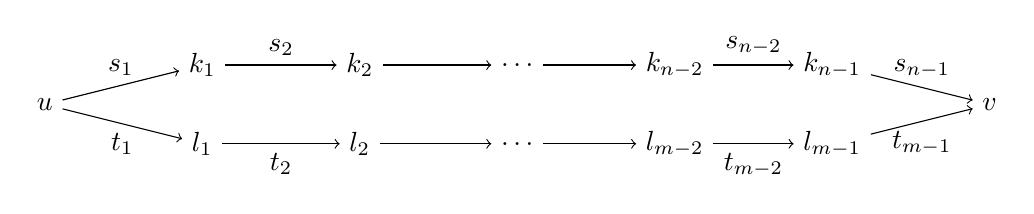
\begin{tikzpicture}
        \node (u) at (0,0) {\( u \)};
        \node (k1) at (2,0.5) {\( k_1 \)};
        \node (k2) at (4,0.5) {\( k_2 \)};
        \node (ketc) at (6,0.5) {\( \dots \)};
        \node (knm2) at (8,0.5) {\( k_{n-2} \)};
        \node (knm1) at (10,0.5) {\( k_{n-1} \)};
        \node (v) at (12,0) {\( v \)};
        \node (l1) at (2,-0.5) {\( l_1 \)};
        \node (l2) at (4,-0.5) {\( l_2 \)};
        \node (letc) at (6,-0.5) {\( \dots \)};
        \node (lnm2) at (8,-0.5) {\( l_{m-2} \)};
        \node (lnm1) at (10,-0.5) {\( l_{m-1} \)};
        \draw[->] (u) -- (k1) node [midway,above] {\( s_1 \)};
        \draw[->] (k1) -- (k2) node [midway,above] {\( s_2 \)};
        \draw[->] (k2) -- (ketc);
        \draw[->] (ketc) -- (knm2); 
        \draw[->] (knm2) -- (knm1) node[midway,above] {\( s_{n-2} \)}; 
        \draw[->] (knm1) -- (v) node[midway,above] {\( s_{n-1} \)}; 
        \draw[->] (u) -- (l1) node[midway,below] {\( t_1 \)};
        \draw[->] (l1) -- (l2) node[midway,below] {\( t_2 \)};
        \draw[->] (l2) -- (letc);
        \draw[->] (letc) -- (lnm2); 
        \draw[->] (lnm2) -- (lnm1) node[midway,below] {\( t_{m-2} \)}; 
        \draw[->] (lnm1) -- (v) node[midway,below] {\( t_{m-1} \)}; 
        \end{tikzpicture}
    }
    \end{center}
    \noindent
    the equality \( h(s_1) \star h(s_2) \star \dots  \star h(s_{n-1}) = h(t_1) \star h(t_2) \star \dots  \star h(t_{m-1}) \) holds.
\end{definition}

\begin{definition}[Pushout \cite{barr1990category}]
    \label{def:cat:po}
    \ \newline
\noindent
\begin{minipage}{0.7\textwidth}  
    A \textbf{pushout} of a span \( B \overset{\alpha}{\leftarrow} A \overset{\beta}{\rightarrow} C \), as shown on the right, is defined as a cospan \( B \overset{\beta'}{\rightarrow} D \overset{\alpha'}{\leftarrow} C \) such that \( \alpha \mathop{\star} \beta' \mathop{=} \beta \mathop{\star} \alpha' \), and for every cospan \( B \overset{\gamma'}{\rightarrow} E \overset{\gamma}{\leftarrow} C \), if \( \alpha \mathop{\star} \gamma' \mathop{=} \beta \mathop{\star} \gamma \) holds, then there exists a unique morphism \(\delta : D \mathop{\to} E\) such that \( \gamma' \mathop{=} \beta' \mathop{\star} \delta \) and \( \gamma \mathop{=} \alpha' \mathop{\star} \delta \).
\end{minipage}
\hfill
\begin{minipage}{0.299\textwidth}
    \hfill
\resizebox{0.9\textwidth}{!}{
           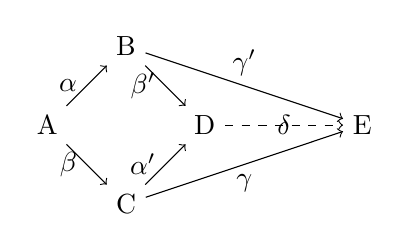
\begin{tikzpicture}
                \node (i) at (0,0) {A};
                \node (r) at (1,1) {B};
                \node (c) at (1,-1) {C};
                \node (h) at (2,0) {D};
                % \node () at (1,-1) {\( \Delta \)};
                \draw[->]  (i) -- (r) node [midway,left] {$ \alpha $};
                \draw[->] (c) -- (h) node [midway,left] {$ \alpha' $};
                \draw[->] (r) -- (h) node[midway, left] {$ \beta' $};
                \draw[->] (i) -- (c) node[midway, left] {$ \beta $};
                \node (d') at (4,0) {E};
                \draw[->] (c) -- (d') node [midway,below]{$ \gamma $};
                \draw[->] (r) -- (d') node [midway,above]{$ \gamma' $};
                \draw[->,dashed] (h) -- (d') node [midway]{$ \delta $};
            \end{tikzpicture}
}
\end{minipage}
The diagram involving \(\alpha\), \(\beta\), \(\alpha'\), and \(\beta'\) is referred to as the \textbf{pushout square}, \(D\) as the \textbf{pushout object}, and the existence of the unique morphism is known as the \textbf{universal mapping property of the pushout}.
\end{definition} 

\begin{definition}[Pullback~\cite{pierce1991basic}]
    \label{def:cat:pb}
    \ \newline
\noindent
\begin{minipage}{0.7\textwidth}  
   A \textbf{pullback} of a cospan \(B \overset{\beta'}{\rightarrow} D \overset{\alpha'}{\leftarrow} C \), as shown on the right, is defined as a span \( B \overset{\alpha}{\leftarrow} A \overset{\beta}{\rightarrow} C \) such that \( \alpha \mathop{\star} \beta' \mathop{=} \beta \mathop{\star} \alpha' \), and for every span \( B \overset{\gamma'}{\leftarrow} E \overset{\gamma}{\rightarrow} C \) if \(\gamma' \mathop{\star} \beta' \mathop{=} \gamma \mathop{\star} \alpha'\) holds, then there exists a unique morphism \(\delta: E \mathop{\to} A\) such that $\gamma' \mathop{=} \delta \mathop{\star} \alpha$ and $\gamma \mathop{=} \delta \mathop{\star} \beta$. 
\end{minipage}
\hfill
\begin{minipage}{0.299\textwidth}
    \hfill
\resizebox{0.9\textwidth}{!}{
            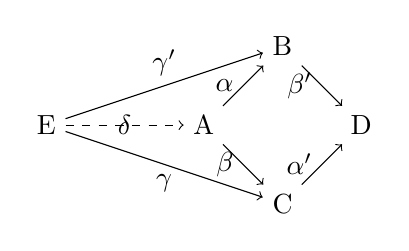
\begin{tikzpicture}
                \node (i) at (0,0) {A};
                \node (r) at (1,1) {B};
                \node (c) at (1,-1) {C};
                \node (h) at (2,0) {D};
                % \node () at (1,-1) {\( \Delta \)};
                \draw[->]  (i) -- (r) node [midway,left] {$\alpha$};
                \draw[->] (c) -- (h) node [midway,left] {$\alpha'$};
                \draw[->] (r) -- (h) node[midway, left] {$\beta'$};
                \draw[->] (i) -- (c) node[midway, left] {$\beta$};
                \node (d') at (-2,0) {E};
                \draw[<-] (c) -- (d') node [midway,below]{$\gamma$};
                \draw[<-] (r) -- (d') node [midway,above]{$\gamma'$};
                \draw[->, dashed] (d') -- (i) node [midway]{$\delta$};
            \end{tikzpicture}
}
\end{minipage}
The diagram involving \(\alpha\), \(\beta\), \(\alpha'\), and \(\beta'\) is referred to as the \textbf{pullback square}, \(A\) as the \textbf{pullback object}, and the existence of the unique morphism is known as the \textbf{universal mapping property of the pullback}.
\end{definition} 
% In the category \(\mathbf{Graph}\) pushouts always exist, and their construction is straightforward when dealing with monomorphisms (injective graph homomorphisms). 
% Let $\uplus$ denote the disjoint union operation. For two sets \(A\) and \(B\), their disjoint union \(A \uplus B\) is defined as the set of ordered pairs \( (x, i) \) where \( x \in A \) if \( i = 1 \) and \( x \in B \) if \( i = 2 \). Formally, we have:
% $
% A \uplus B = \{ (x, 1) : x \in A \} \cup \{ (x, 2) : x \in B \}.
% $ 
We denote $X\uplus Y$ the union of two disjoint sets. By possibly renaming nodes, a span of injective graph homomorphisms can be represented as
$
A \uplus B' \overset{\alpha}{\leftarrowtail} A \overset{\beta}{\rightarrowtail} A \uplus C'
$
where $A,B',C'$ are disjoint sets and $\alpha$ and $\beta$ are inclusion function. A pushout of this span is then given by
$
A \uplus B'  \overset{\beta'}{\rightarrowtail} A \uplus B' \uplus C'   \overset{\alpha'}{\leftarrowtail} A \uplus C'
$ where $\alpha'$ and $\beta'$ are inclusion function. This situation can be depicted by the diagram in \autoref{fig:po_decomp}
\begin{figure}[htbp] 
    \begin{center}
    \resizebox{0.45\textwidth}{!}{
        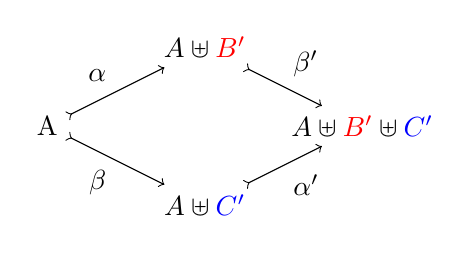
\begin{tikzpicture}
                    \node (i) at (0,0) {A};
                    \node (r) at (2,1) {$A \uplus \textcolor{red}{B'}$};
                    \node (c) at (2,-1) {$A \uplus \textcolor{blue}{C'}$};
                    \node (h) at (4,0) {$A \uplus \textcolor{red}{B'} \uplus \textcolor{blue}{C'}$};
                    \draw[>->]  (i) -- (r) node [midway, above left] {$\alpha$};
                    \draw[>->] (c) -- (h) node [midway, below right] {$\alpha'$};
                    \draw[>->] (r) -- (h) node[midway, above right] {$\beta'$};
                    \draw[>->] (i) -- (c) node[midway, below left] {$\beta$};
        \end{tikzpicture}
    }
    \end{center}
    
    \caption{Construction of the pushout of a span of monomorphisms in \(\mathbf{Graph}\)}
    \label{fig:po_decomp}
\end{figure}
where \(B'\) and \(C'\) are colored to make evident this decomposition in a concrete example within \textbf{Graph} in \autoref{ex:po_in_graph}, where nodes and arrows are colored accordingly.

% %po example in Graph
% \begin{example}
    \label{ex:po_in_graph}
    The following diagram
    %  in Figure~\ref{fig:ex:po_in_graph} 

% \begin{figure}[H] 
\begin{center}
    \resizebox{0.5\textwidth}{!}{
        \begin{tikzpicture}
               
                \graphbox{ }{40mm}{5mm}{34mm}{15mm}{2mm}{0mm}{
                    \coordinate (o) at (0mm,-8mm); 
                    \node[draw,circle] (l1) at ($(o)+(-10mm,0mm)$) {1};
                    \node[draw,circle] (l2) at ($(l1)+(2,0)$) {2};
                }  
  
                \graphbox{ }{80mm}{5mm}{45mm}{15mm}{2mm}{-0mm}{
                    \coordinate (o) at (-5mm,-8mm); 
                    \node[draw,circle] (l1) at ($(o)+(-10mm,0mm)$) {1};
                    \node[draw,circle] (l2) at ($(l1)+(3,0)$) {2};
                    \node[red,draw,circle] (l3) at ($(l1)+(1,0)$) {4};
                    \node[red,draw,circle] (l4) at ($(l1)+(2,0)$) {5};
                    \draw[red] (l1) -- (l3) node[midway,above] {$a$};
                    \draw[red] (l3) -- (l4) node[midway,above] {$b$};
                    \draw[red] (l4) -- (l2) node[midway,above] {$a$};
                }    
                \graphbox{ }{40mm}{-17mm}{34mm}{25mm}{2mm}{-5mm}{
                    \coordinate (o) at (0mm,-3mm); 
                    \node[draw,circle] (l1) at ($(o)+(-10mm,0mm)$) {1};
                    \node[draw,circle] (l2) at ($(l1)+(2,0)$) {2};
                    \node[blue,draw,circle] (l4) at ($(l2)+(0,-1)$) {6};
                    \draw[blue] (l2) -- (l4) node[midway,right] {$a$};
                    \node[blue,draw,circle] (l6) at ($(l1)+(0,-1)$) {7};
                    \draw[blue] (l1) -- (l6) node[midway,left] {$a$};
                }    
  
                \graphbox{ }{80mm}{-17mm}{45mm}{25mm}{2mm}{-5mm}{
                    \coordinate (o) at (-5mm,-3mm); 
                    \node[draw,circle] (l1) at ($(o)+(-10mm,0mm)$) {1};
                    \node[draw,circle] (l2) at ($(l1)+(3,0)$) {2};
                    \node[draw,circle,red] (l3) at ($(l1)+(1,0)$) {4};
                    \node[draw,circle,red] (l4) at ($(l1)+(2,0)$) {5};
                    \node[blue,draw,circle] (l5) at ($(l2)+(0,-1)$) {6};
                    \node[blue,draw,circle] (l6) at ($(l1)+(0,-1)$) {7};
                    \draw[blue] (l1) -- (l6) node[midway,left] {$a$};
                    \draw[red] (l1) -- (l3) node[midway,above] {$a$};
                    \draw[red] (l3) -- (l4) node[midway,above] {$b$};
                    \draw[red] (l4) -- (l2) node[midway,above] {$a$};
                    \draw[blue] (l2) -- (l5) node[midway,right] {$a$};
                }    
  
                \node () at (77mm,-3mm) {\( \rightarrowtail \)}; % K -> R
                \node () at (52mm,-13mm) {\( \downarrowtail \)};
                \node () at (92mm,-13mm) {\( \downarrowtail \)};
                \node () at (77mm,-28mm) {\( \rightarrowtail \)}; % C -> H
        \end{tikzpicture}
    }
\end{center}
% \caption{Example of the pushout of span of monomorphism in \(\mathbf{Graph}\)}
% \label{fig:ex:po_in_graph}
% \end{figure}
     is a pushout square in the category \textbf{Graph} where nodes and arrows are colored to visualize the decomposition as in Figure~\ref{fig:po_decomp}.
\end{example}

To demonstrate that the diagram above is a pushout square, consider an object \( X \) and morphisms \( f: A \uplus B' \mathop{\to} X \) and \( g: A \uplus C' \mathop{\to} X \) such that \( \alpha \mathop{\star} f \mathop{=} \beta \mathop{\star} g \). Since \( \alpha \) and \( \beta \) are inclusion maps, it follows that \( f \) and \( g \) agree on \( A \). Therefore, the morphism \( h: A \uplus B' \uplus C' \mathop{\to} X \) defined by $h(x) \mathop{=} f(x)$ if $x\in A\uplus B'$ and $h(x) \mathop{=} g(x)$ otherwise is the unique morphism such that $\beta' \mathop{\star} h \mathop{=} f$ and $\alpha' \mathop{\star} h \mathop{=} g$. Thus, the object \( A \uplus B' \uplus C' \), together with the morphisms \( \beta' \) and \( \alpha' \), satisfies the universal property of the pushout. Furthermore, the compositions \( \alpha \mathop{\star} \beta'\) and \( \beta \mathop{\star} \alpha'\) both map elements from \( A \) to \( A \uplus B' \uplus C' \) via inclusion function.
Since all maps are inclusions and \( A \), \( B' \), and \( C' \) are disjoint, the square commutes $
     \alpha \mathop{\star} \beta' \mathop{=} \beta \mathop{\star} \alpha'
$. Therefore, the diagram is indeed a pushout square.
%pb po in Grap
\begin{notation}
    When the context makes it clear, a morphism \( h : A \mathop{\to} B \) will be denoted by \( h_{AB} \), and diagrams will be referred to by their nodes, as is standard in geometry. For example, the diagram involving the morphisms \( \alpha, \beta, \alpha', \beta' \) in Definition~\ref{def:cat:po} will be denoted by \( ACDB \) or \( ABDC \).
\end{notation}   
\begin{remark}
    We work within the category \textbf{Graph}. The terms homomorphism and morphism will be used interchangeably; the same applies to monic and injective, and to injective homomorphism and monomorphism.
\end{remark}